% chap3.tex - Week 3
\cleardoublepage
%\phantomsection

%% TODO - quick checkout / branch create in breakout

\chapter{Week 3}
\section{Day 1 - ``But how do I see what's going on?''}
\subsection{Logging in Git}

Perhaps the best feature of a version control system is the level of accountability that it offers if set up correctly.  What do we mean by this?  People often mistake the word \textbf{accountability} for the word \textbf{blame}.  This is not true at all.  Accountability is key in understanding the events that led up to a particular bug being introduced, or a situation occurring.  How this is dealt with, is a up to the management teams, but accountability should not be something that is revered, it should be something that is looked upon as a tool to help define the cause of a problem.

By its very nature, a version control system is also a logging system.  Every time we committed something into the repository in the last chapter, we supplied a log message.  In fact, if we don't supply a commit message, let us see what happens.

\begin{Verbatim}[frame=leftline,framerule=1mm,fontsize=\relsize{-3}] 
john@akira:~/coderepo$ git status
# On branch master
# Untracked files:
#   (use "git add <file>..." to include in what will be 
committed)
#
#	my_third_committed_file
nothing added to commit but untracked files present (use "git 
add" to track)
john@akira:~/coderepo$ git add my_third_committed_file
john@akira:~/coderepo$ git commit -a -m ''
Aborting commit due to empty commit message.
john@akira:~/coderepo$ 
\end{Verbatim}

Git will actually not allow you to commit with a blank message.  This is actually fantastic news, as people are far less likely to write a useless message than they are a blank one.  It is very important that when using a version control system you write in a useful commit message.  If you fixed a bug, say so.  If you added a new function, why not put that in too.  When someone wants to find out what a certain commit was for, or even when you come back to the project six months later and realise you've forgotten everything, log messages are crucial in piecing back together a history of development.

\begin{trenches}
``So John, I've been committing and all that,'' started Rob, ``but how do I see the history of what I have done.''

``It's really pretty simple,'' replied John, ``But it really depends on what you want to know.''
Rob placed his thumb and forefinger onto his chin.  ``Well, for now, I just want to see a list of all of my commits.''

``That one's the simplest of all.''
\end{trenches}

At its simplest, \texttt{git log} will give an output of all of the commits that have been applied to the current branch.  Depending on what type of machine you are using it on, the output from \texttt{git log} will be navigable, usually using the up and down arrows, with 'q' used to quit.  Let's have a quick look at the output of our test repository and see what the log messages look like.

\begin{Verbatim}[frame=leftline,framerule=1mm,fontsize=\relsize{-3}] 
john@akira:~/coderepo$ git log
commit 6ca160c7226731bf80973fc5bc81f6b9beda7795
Author: John Haskins <john.haskins@tamagoyakiinc.koala>
Date:   Mon Feb 21 20:59:32 2011 +0000

    Finished adding initial files

commit e86ddea25341a75275d316d8ca545aa7c73e97b3
Author: John Haskins <john.haskins@tamagoyakiinc.koala>
Date:   Mon Feb 21 20:06:57 2011 +0000

    Made a few changes to first and second files

commit 88206926cb60aed53d21ede69f9ca5b7c69cb983
Author: John Haskins <john.haskins@tamagoyakiinc.koala>
Date:   Sat Feb 19 09:23:47 2011 +0000

    My First Ever Commit
john@akira:~/coderepo$ 
\end{Verbatim}

The \texttt{git log} command shows us a chronological list of all of the commits to the repository and also gives us several more important pieces of information.  In total there are four pieces of information displayed by default.

\begin{itemize}
\item \textbf{commit} - This is the SHA-1 hash of the commit object that is stored inside the repository.  You can find more information about this in the \emph{What's inside the Git repository?} section \emph{Week 2}.  This is how we refer to the commit.  If someone asked you in what commit you \emph{Made a few changes to first and second files}, you could reply that you did that in commit e86dd.  As explained earlier, it is good to remember that you don't need to remember or type out the whole \textbf{e86ddea25341a75275d316d8ca545aa7c73e97b3}, only the first part is required.  Generally, the first five characters will do.
\item \textbf{Author} - This is the name and email address of the author of the commit.  When we begin to look at merging, you will see that the author of a commit, is not necessarily the \emph{committer} of the commit.  If you want to find out more about how to set these options, see the breakout box in this Week, called \emph{Changing your identity}.
\item \textbf{Date} - The date is simply the date at which the commit was created.  Again, note that when we start looking at merging, the date will be the date the commit was created, not the date it was merged into the repository.
\item \textbf{Commit Message} - This is the log message that was added along with the commit when it was created.  Hopefully you can now see how important it is to create useful and meaningful messages in here.
\end{itemize}

\begin{figure}[hbt]
\tikzstyle{mybox} = [draw=black, fill=gray!20, very thick, rectangle, rounded corners, inner sep=15pt, inner ysep=20pt]
\tikzstyle{fancytitle} =[fill=black, text=white]
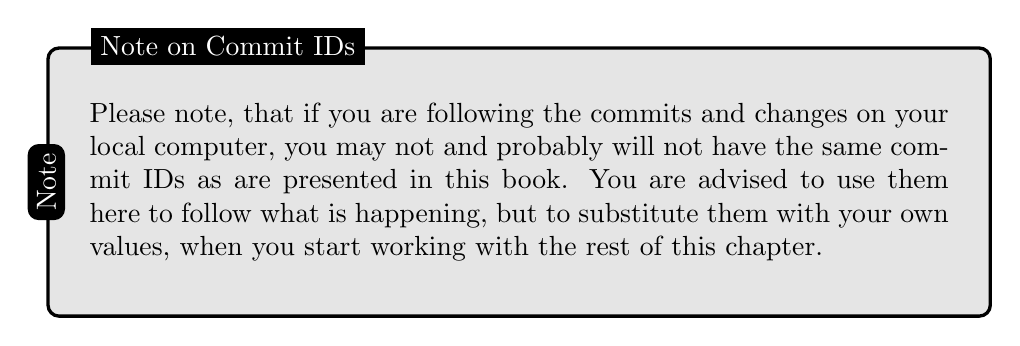
\begin{tikzpicture}
\node [mybox] (box){%
    \begin{minipage}{.9\textwidth}
Please note, that if you are following the commits and changes on your local computer, you may not and probably will not have the same commit IDs as are presented in this book.  You are advised to use them here to follow what is happening, but to substitute them with your own values, when you start working with the rest of this chapter.
    \end{minipage}
};
\node[fancytitle, right=16pt] at (box.north west) {Note on Commit IDs};
\node[fancytitle, rounded corners] at (box.west) {\rotatebox{90}{Note}};
\end{tikzpicture}
\end{figure}

\begin{figure}[hbt]
\tikzstyle{mybox} = [draw=black, fill=gray!20, very thick, rectangle, rounded corners, inner sep=15pt, inner ysep=20pt]
\tikzstyle{fancytitle} =[fill=black, text=white]
\begin{tikzpicture}
\node [mybox] (box){%
    \begin{minipage}{.9\textwidth}
Particularly when working with other people, or when publishing your repository to a public location, it's a good idea to make sure people know who you are and how to get in contact with you.  Every time you make a commit to a repository, Git gives the opportunity to take note of who posted the commit.  When you first install Git, it probably won't have the correct information in there for you, so it's important that you take the time to set this up.

To set up your name and email address, we need to modify the \texttt{gitconfig} again.  

\begin{Verbatim}[frame=leftline,framerule=1mm,fontsize=\relsize{-3}] 
$ git config --global user.name "John Haskins"
$ git config --global user.email 
"john.haskins@tamagoyakiinc.koala"
\end{Verbatim}

That's it.  Now by default, Git will use this setting whenever you commit to a repository, unless you override it by locally modifying the repository's \texttt{.gitconfig}.
    \end{minipage}
};
\node[fancytitle, right=16pt] at (box.north west) {Changing your identity};
\node[fancytitle, rounded corners] at (box.west) {\rotatebox{90}{Note}};
\end{tikzpicture}
\end{figure}

\section{Day 2 - ``But I need more information''}
\subsection{Digging a little deeper}

\begin{trenches}
``I know John, and next time I will make a note of it, but right now, I'd really like to know where this file got changed,'' Klaus pointed at the piece of paper containing a print out, ``specifically when this function was introduced.''

John smiled.  His hands danced over the keyboard as he finished compiling an email.  ``And you've no idea when this was added at all?'' he asked.

``No, sorry John, I don't.''  He pondered, ``I guess I could write a script to untar all the versions we've created in the last week and search through them.''  He sighed, ``Can't the wonderful Git help us out here?''

A head popped up over the cubicle wall.  ``You wanna find out when a function was introduced to a file?''  It was Rob.  ``After John showed me the basics, I went and read up on it a little.  Git has some really powerful searching within the log tool.''

``Well come on then,'' blurted Klaus, ``Don't keep me hanging on.''

A chime of the popular 1966 hit sprang out in the office.

Klaus pulled a hand down over his face, ``Oh don't you all start!''
\end{trenches}

Git can actually do some rather powerful searching to assist a developer in their daily tasks.  It would have been useful if the particular item that was being searched for had been included in the log, but sometimes, things either get missed, or there are just too many changes introduced in one commit to list them all.

In these instances, the \texttt{git log -S<string>} command comes to our aid.  This command will search through the commits in a repository and will return a list of commits which introduced or removed a specific string into the repository.  First of all, let's run this against our test repository.

\begin{Verbatim}[frame=leftline,framerule=1mm,fontsize=\relsize{-3}] 
john@akira:~/coderepo$ git log -SChange1
commit e86ddea25341a75275d316d8ca545aa7c73e97b3
Author: John Haskins <john.haskins@tamagoyakiinc.koala>
Date:   Mon Feb 21 20:06:57 2011 +0000

    Made a few changes to first and second files
john@akira:~/coderepo$ 
\end{Verbatim}

You can see that \texttt{git log} has shown us the commit that instantiated the change.  As you can imagine, when using a large code base, this tool can be invaluable.  It allows us to pinpoint a specific moment when a certain string of text entered the repository.  When running this against a very large repository, this could take a long time, and so the ability to shrink the search scope down will result in a much faster result.  To do this we can append a path to our previous command.  

\begin{Verbatim}[frame=leftline,framerule=1mm,fontsize=\relsize{-3}] 
john@akira:~/coderepo$ git log -SChange2 my_first_committed_file
john@akira:~/coderepo$ git log -SChange2 my_second_committed_file
commit 6ca160c7226731bf80973fc5bc81f6b9beda7795
Author: John Haskins <john.haskins@tamagoyakiinc.koala>
Date:   Mon Feb 21 20:59:32 2011 +0000

    Finished adding initial files
john@akira:~/coderepo$ 
\end{Verbatim}

If you remember from our committing back in Week 2, we added the string \texttt{Change2} to the second file but not the first.  So the first time we run this command, it fails, as we are searching against \texttt{my\_first\_committed\_file}.  The second time we run it, we are searching against \texttt{my\_second\_committed\_file} and this is where we see a result.  Commit 6ca16 contains the commit we are looking for.

\section{Day 3 - ``What actually changed?''}
\subsection{Doing the diff dance}

Knowing what the committer thinks they committed is brilliant.  However, sometimes it's just not enough.  The reason for this is stated fairly precisely in the first sentence of this paragraph, so let us add a little formatting to bring out the real meaning.  Knowing what the committer \emph{thinks} they committed is brilliant.  By looking at the commit message we only know as much as the committer wants us to.  If they are the helpful sort, this will probably be all that we need, most of the time.  On the other hand there is always the situation where you'd like to know a little more about what was actually placed into the repository.

The \texttt{git diff} command can show us exactly that.  For more information about diff in general, see the diff breakout box in this chapter.  Think of a diff as an easy way of looking at the differences between two files, surrounded by a little context.  This can often be enhanced by a visual diff viewer, but for now, let's stick with our simple text based \texttt{git diff}.  

If we want to find out what the changes are between our current commit and one of the previous ones, we can write a command like the one below.  Notice that below, \textbf{e86dd} refers to the second commit that we made to the repository.  

\begin{Verbatim}[frame=leftline,framerule=1mm,fontsize=\relsize{-3}] 
john@akira:~/coderepo$ git diff e86dd
diff --git a/my_second_committed_file b/my_second_committed_file
index 3ad4cc3..095b9cd 100644
--- a/my_second_committed_file
+++ b/my_second_committed_file
@@ -1 +1,2 @@
 Change1
+Change2
john@akira:~/coderepo$ 
\end{Verbatim}

What this is telling us, is that between \textbf{e86dd} and our current commit \textbf{6ca16}, we added the line \emph{Change2} to the file \texttt{my\_second\_committed\_file}.  We can see this by the preceding \texttt{+} on the line \texttt{Change2}.  Let's make a few changes to our repository and see how the diffs look.  We're actually going to make a few changes to the files using a text editor so that you can't see what we've done.  Then, hopefully, when we run the \texttt{git diff} you'll be able to see clearly what has happened.

\begin{Verbatim}[frame=leftline,framerule=1mm,fontsize=\relsize{-3}] 
john@akira:~/coderepo$ git log HEAD~1..HEAD
commit fa65f06cc62291bb0cd47aef9e05953d6655fc8e
Author: John Haskins <john.haskins@tamagoyakiinc.koala>
Date:   Tue Mar 1 21:17:57 2011 +0000

    Messed with a few files
john@akira:~/coderepo$ 
\end{Verbatim}

The command \texttt{git log HEAD\textasciitilde1..HEAD} tells Git to show us the git log for all commits between \texttt{HEAD~1} and \texttt{HEAD}.  The notation used here is something new to us, but seeing as HEAD points to the most current commit, HEAD~1 points to the commit previous to HEAD.  This is how we tell Git to show us only the most recently commit.  

As it turns out, John Haskins didn't really create a very meaningful log message.  \emph{Messed with a few files} is pretty unhelpful in the grand scheme of things.  So let's be thankful that this isn't Tamagoyaki Inc's core repository and take a look at what actually happened in the commit \textbf{fa65f}.

\begin{Verbatim}[frame=leftline,framerule=1mm,fontsize=\relsize{-3}] 
john@akira:~/coderepo$ git diff HEAD~1..HEAD
diff --git a/my_second_committed_file b/my_second_committed_file
index 095b9cd..c9887f8 100644
--- a/my_second_committed_file
+++ b/my_second_committed_file
@@ -1,2 +1 @@
-Change1
-Change2
+Changed this file completely
diff --git a/my_third_committed_file b/my_third_committed_file
new file mode 100644
index 0000000..5d27866
--- /dev/null
+++ b/my_third_committed_file
@@ -0,0 +1 @@
+Addition to the line
john@akira:~/coderepo$ 
\end{Verbatim}

As you can see, we have several things going on here, so let's take each of them in isolation and see what is going on.  We are going to dissect the diff to see what each section means.

\begin{Verbatim}[frame=leftline,framerule=1mm,fontsize=\relsize{-3}] 
diff --git a/my_second_committed_file b/my_second_committed_file
\end{Verbatim}

This first line tells us that we are dealing with \texttt{my\_second\_committed\_file}.  This is showing that we are comparing the first revision, or a, against the second revision, b.

\begin{Verbatim}[frame=leftline,framerule=1mm,fontsize=\relsize{-3}] 
index 095b9cd..c9887f8 100644
\end{Verbatim}

This second line actually tells us the beginning of the object IDs, as they are stored in the repository.  Note that these IDs are not the commit IDs, but the actual blob IDs that Git uses to refer to the file.  For more information on this, checkout the \emph{Object's living in harmony} breakout box.

\begin{Verbatim}[frame=leftline,framerule=1mm,fontsize=\relsize{-3}] 
--- a/my_second_committed_file
+++ b/my_second_committed_file
\end{Verbatim}

The next few lines are telling us which is the original file, and which is the new file, so we can use this as a reference.

\begin{Verbatim}[frame=leftline,framerule=1mm,fontsize=\relsize{-3}] 
@@ -1,2 +1 @@
-Change1
-Change2
+Changed this file completely
\end{Verbatim}

Now we see some lines which are generally referred to as a hunk.  The hunk has two important pieces of information.  Section \texttt{-1,2} tells us that in the original file, we are looking at the original file (\texttt{-}), that the starting line where the change takes place is line 1 (\texttt{1}) and that the hunk applies to two lines (\texttt{2}).  The next section tells us that in the new file, the change takes place as line 1, and because the comma and remaining number are omitted, we can infer that the hunk applies to only 1 line.

The three following lines show what actually took place.  Strings \texttt{Change1} and \texttt{Change2} were deleted from the file, whereas \texttt{Changed this file completely} was added to the file.

Looking at the next diff segment, we can see it applies to a different file.  Essentially this hunk is no different to the last, the only interesting portion is shown below.

\begin{Verbatim}[frame=leftline,framerule=1mm,fontsize=\relsize{-3}] 
new file mode 100644
index 0000000..5d27866
--- /dev/null
+++ b/my_third_committed_file
\end{Verbatim}

This shows us that \texttt{my\_third\_committed\_file} is actually a new file.  Notice the \texttt{/dev/null} and the \texttt{0000000} object ID, indicating that there was no original file.

\subsection{Diffing Over A Range}
All the operations that we have performed so far have been on one commit.  Whilst important and valuable, it may be that you want to see an entire range of changes.  

\begin{trenches}
``I'm still not entirely convinced about this John,'' said Martha.  ``I've been playing around with Git, like you asked me, but it still just seems like we're replicating the work that we used to do with the readme changelogs and the tarball files.''

She sat down on a near-by chair and wheeled it over to John's desk.  She surveryed the desk for an inch of vacant real estate before finally resting her elbow on the corner of his desk next to a copy of Pro Git.

``Well, actually Martha, I can see exactly what you mean.  Up until now, there is no difference between the old and the new process.  I'm still in control of all the versions, so nothing has really changed.''  He thought long and hard, ``Tell ya what.  Why don't you give me an operation that you've always wanted to do against our code tree tarballs easily.''

``Easy,'' she snapped back, ``I want to know what changes were made for the last two weeks whilst I had been away on holiday.'' She smiled an almost mischievous smile as she referenced 'The Incident', as it had become known throughout the office.

``Easy,'' John quipped, mimicking her mannerisms.  The two broke out in laughter.  ``We can use git log for that, and I think there are some date options too.  Let me check the man page.''
\end{trenches}

Looking at the man page for git log is a mind trip for the uninitiated.  Weighing in at over 600 lines of text, it is abundantly clear that this tool does a whole lot more than viewing a simple history of commits to the repository.  It is well worth taking the time to read through the current available options by typing \texttt{man git log} on the command line.  If you have the documentation installed, this will yield the \emph{man} page for \texttt{git log}.

Listing all commits in our repository is useful, being able to filter this output is fantastic.  This is one area in which the developers of Git have placed a great deal of time and effort.  For example, we can use \texttt{git log} to not only show us the commit message, but also provide a diff output as well.  This means that for each commit entry in the output, we will see a diff as well.  Now, whilst we are further empowered by having the diff output in chronological order for each commit, we can take things further by filtering the commits.  

Suppose we want to view all the commits that we made in the last week, typing the following into the command line in our test repository yields the following result.

\begin{Verbatim}[frame=leftline,framerule=1mm,fontsize=\relsize{-3}] 
john@akira:~/coderepo$ git log -p --since="last week"
commit fa65f06cc62291bb0cd47aef9e05953d6655fc8e
Author: John Haskins <john.haskins@tamagoyakiinc.koala>
Date:   Tue Mar 1 21:17:57 2011 +0000

    Messed with a few files

diff --git a/my_second_committed_file b/my_second_committed_file
index 095b9cd..c9887f8 100644
--- a/my_second_committed_file
+++ b/my_second_committed_file
@@ -1,2 +1 @@
-Change1
-Change2
+Changed this file completely
diff --git a/my_third_committed_file b/my_third_committed_file
new file mode 100644
index 0000000..5d27866
--- /dev/null
+++ b/my_third_committed_file
@@ -0,0 +1 @@
+Addition to the line
john@akira:~/coderepo$ 
\end{Verbatim}

Notice we get to see the diff that was presented before when we ran our \texttt{git diff HEAD\textasciitilde1..HEAD} command, but this time, as we have used the git log command instead, we get to see the diff output as well.  This is what the \texttt{-p} flag is for.  Take note of the way we have specified the time period that we are interested in.  The section \texttt{--since="last week"} tells Git to filter the output and show only the entries that were committed within the last week.

This type of filtering can be exceedingly useful to a developer.  Often when problems arise, you do not have a defined point in time that you know it was last working.  However most of the time, you can say with some certainty, ``I know it was working two weeks ago''.  Using the methods described above, will give the user all of the changes, categorised by commit, that occurred in those two weeks, allowing them to narrow down the scope of exactly where to begin looking for the offending changes.

If the developer can further categorise the issue, such as, ``I know which file the change must have occurred in'', then the following example will demonstrate just how easy it is to filter the results even further.  Even in the simplified example repository that we have been using, running this command filters the output to a single file.

\begin{Verbatim}[frame=leftline,framerule=1mm,fontsize=\relsize{-3}] 
john@akira:~/coderepo$ git log -p --since="last week" -- 
my_second_committed_file
commit fa65f06cc62291bb0cd47aef9e05953d6655fc8e
Author: John Haskins <john.haskins@tamagoyakiinc.koala>
Date:   Tue Mar 1 21:17:57 2011 +0000

    Messed with a few files

diff --git a/my_second_committed_file b/my_second_committed_file
index 095b9cd..c9887f8 100644
--- a/my_second_committed_file
+++ b/my_second_committed_file
@@ -1,2 +1 @@
-Change1
-Change2
+Changed this file completely
john@akira:~/coderepo$ 
\end{Verbatim}

See how easy that is.  Note, the \texttt{--} is necessary to tell Git the following string is a path.  We no longer have the information for \texttt{my\_third\_committed\_file} present in the output.  We have filtered everything out but the information we are looking for.  When you are up against deadlines, pouring through pages and pages of diffs and changes can be incredibly time consuming.  Having the tools available to cut that output down to just the relevant material can be life saving.

\section{Day 4 - ``Finding a good reference point''}
\subsection{Tag you're it!}

During software development, a project will generally get to a point where it is ready to be released to people outside of the development team.  When this grand day occurs, it is crucial that both the developers and the users have a reference point with which to refer to the state of the code.  Having a code name or a version number means that within a very short period of time, both parties can converse about a problem, safe in the knowledge that they are on the same page.

In most version control systems, the word tagging is used to describe a reference point in the code's history.  A tag will usually refer to a single commit and labels that particular commit with a name that is easier to remember than a standard version number or SHA-1 hash.  The tag name used can be a codename, or a version number.  Often people will follow a simple numbering scheme, like \texttt{v1.9}.  

In this example, the \texttt{1} may refer to the major version number, and will denote a family of versions, often only changing a few times in a projects lifetime.  The \texttt{9} is a minor version number and can refer to a much more frequent release schedule.  You may also see textual items being appended to this version string, like \texttt{rc}, \texttt{b}, and \texttt{a}, denoting \emph{Release Candidate}, \emph{Beta} and \emph{Alpha} respectively.

Git implements tags in a very elegant way.  A tag is simply a label in Git that points to a single commit object.  The tag name can then be used in place of the SHA-1 to refer to a point in the repositories history.  Due to the simplicity of tags, it is also possible and very simple to tag a commit that occurred way into the past.  Let us take a look at a simple tag example.  We will make the current point in the repository \texttt{v1.0a}.

\begin{Verbatim}[frame=leftline,framerule=1mm,fontsize=\relsize{-3}] 
john@akira:~/coderepo$ git tag v1.0a
john@akira:~/coderepo$ 
\end{Verbatim}

On its own, this doesn't really tell us much, but running the following, shows us a little more information

\begin{Verbatim}[frame=leftline,framerule=1mm,fontsize=\relsize{-3}] 
john@akira:~/coderepo$ git rev-parse v1.0a
fa65f06cc62291bb0cd47aef9e05953d6655fc8e
john@akira:~/coderepo$ 
\end{Verbatim}

By running the \texttt{git rev-parse} with the tag name \texttt{v1.0a}, Git has returned us the SHA-1 hash of the commit we were referring to.  If we look back up at the earlier output, we can see that the most recent commit into the repository was indeed \textbf{fa65f06cc62291bb0cd47aef9e05953d6655fc8e}.  To give us something to work with, let's tag the commit \textbf{e86dd\ldots} with the tag name \texttt{v0.9}.

\begin{Verbatim}[frame=leftline,framerule=1mm,fontsize=\relsize{-3}] 
john@akira:~/coderepo$ git tag v0.9 e86dd
john@akira:~/coderepo$ 
\end{Verbatim}

Now, we can do the following;

\begin{Verbatim}[frame=leftline,framerule=1mm,fontsize=\relsize{-3}] 
john@akira:~/coderepo$ git diff v0.9..v1.0a
diff --git a/my_second_committed_file b/my_second_committed_file
index 3ad4cc3..c9887f8 100644
--- a/my_second_committed_file
+++ b/my_second_committed_file
@@ -1 +1 @@
-Change1
+Changed this file completely
diff --git a/my_third_committed_file b/my_third_committed_file
new file mode 100644
index 0000000..5d27866
--- /dev/null
+++ b/my_third_committed_file
@@ -0,0 +1 @@
+Addition to the line
john@akira:~/coderepo$ 
\end{Verbatim}

Notice that instead of using the dynamic reference HEAD, we have now used the tag names \texttt{v0.9} and \texttt{v1.0a} to refer to our previous commits and have returned the combined diff output of all the changes which occurred between the two.

You can find out more about tags and how to specify more information in the \emph{After Hours} section at the end of this Week.

\begin{figure}[hbt]
\tikzstyle{mybox} = [draw=black, fill=gray!20, very thick, rectangle, rounded corners, inner sep=15pt, inner ysep=20pt]
\tikzstyle{fancytitle} =[fill=black, text=white]
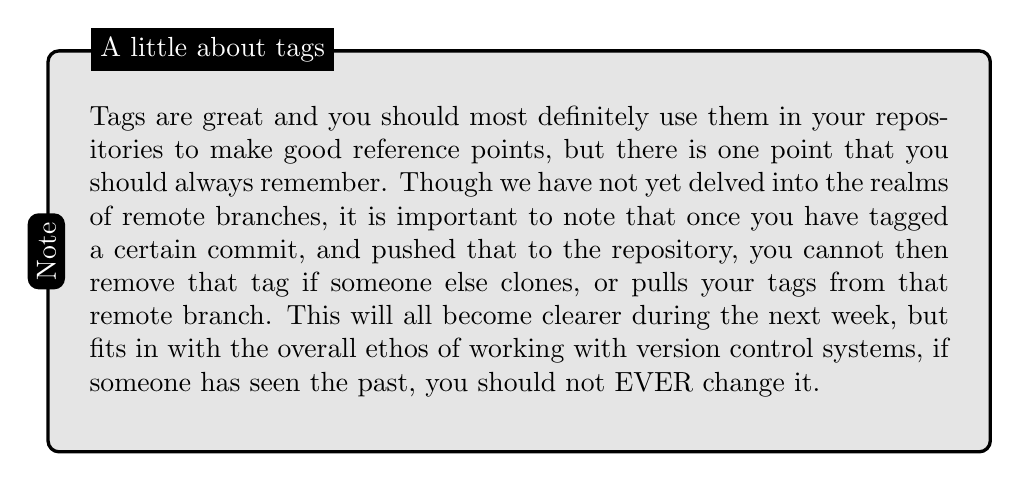
\begin{tikzpicture}
\node [mybox] (box){%
    \begin{minipage}{.9\textwidth}
Tags are great and you should most definitely use them in your repositories to make good reference points, but there is one point that you should always remember.  Though we have not yet delved into the realms of remote branches, it is important to note that once you have tagged a certain commit, and pushed that to the repository, you cannot then remove that tag if someone else clones, or pulls your tags from that remote branch.  This will all become clearer during the next week, but fits in with the overall ethos of working with version control systems, if someone has seen the past, you should not EVER change it.
    \end{minipage}
};
\node[fancytitle, right=16pt] at (box.north west) {A little about tags};
\node[fancytitle, rounded corners] at (box.west) {\rotatebox{90}{Note}};
\end{tikzpicture}
\end{figure}

\section{Day 5 - ``Putting things back the way they were''}
\subsection{Revert, I say.  Revert!}

Whilst working with your repository, something occurs quite often, is the need to go back in time, either temporarily or permanently, or even partially.  Git allows you to do this in a multitude of ways.  Let's see a real life situation where this need could arise.

\begin{trenches}
``No, I don't have a copy of the file.  I was stupid and after I submitted it to you I er\ldots\deleted it''.  

John gave Michael the raised eyebrow look.  It wasn't the first time Michael had come to him with a similar problem.  Usually John would have had Michael go rooting through the archives to find it.  This time though, he wondered if Git might just come to the rescue.

``Tell ya what Michael,'' he grinned, ``Since this isn't the first time you've come to me with this kind of predicament, why don't you go and find out how to use Git to get the file back.''  Michael sighed.  ``I have tagged the repo each time we created an archive, so tell me what I need to run to extract it.''

\begin{center} * * * \end{center}

``Man'', started Michael running over to John's desk forty five minutes later.  ``I never knew there were so many ways to skin a cat''

Michael was a little out of shape and though he had only crossed a minor distance, he now stood there, leaned over John's desk ever so slightly out of breath.

``So, you learn much?'' asked John.

``Where d'ya want me to start?''

\end{trenches}

Where exactly do we start?  Well one of the neat things about Git is that there are many ways to produce the same result.  While that may not seem like a benefit now, the trick is knowing just how to use each tool and what the benefit is of each method.  Right now, we are ready to look at four methods for achieving the task of viewing old information in the repository.  So how do we choose which method we wish to use?  We need to answer a few more questions before we are ready to decide.

The table below shows the three methods that we have access to now.  Note that this may not be a definitive list of methods, but that these can give us access to the data we need to view.  The columns are requirements or criteria.  We need to evaluate each command in order to determine which one is right for us.  Once you have been using Git a while, these kind of evaluations will become second nature to you, but right now, we will take a look at all available options, just to see what is out there.

\begin{table}
\begin{center}
  \begin{tabular}{ | l | l | l | l | l | l |}
    \hline
    Method Name & 
    \rotatebox{90}{Alters Repository} & 
    \rotatebox{90}{Changes History} &
    \rotatebox{90}{Alters Working Copy} & 
    \rotatebox{90}{Reversible} & 
    \rotatebox{90}{Multiple Files} \\ \hline
    Reset & Possibly & Possibly & Possibly & Possibly & Yes\\ \hline
    Checkout & No & No & Yes & No & Yes\\ \hline
    Show & No & No & No & N/A & No\\ \hline
  \end{tabular}
\end{center}
\end{table}

Let's take a look at each of these in turn.  We are going to be covering two new commands and revisiting an old one.  Let us start with \texttt{git reset}.  We have already met this tool once.  When we used it previously, its purpose was to pull files out of the index that we were not ready to commit.  We were using \texttt{git reset} in its simplest state.  Actually Git can perform several other kinds of reset.  It should be noted here that using this can be quite dangerous as it can affect your index, your working copy, your branch and the pointer HEAD.  

In order to use \texttt{git reset} in any sane way to achieve our goal, we would need to look at branching, which at the moment, we are not ready to do.  In short \texttt{git reset} can drastically effect your working copy, affecting multiple files, and before we begin investigating, we really need to learn how to play in a safe environment.  

The next method on our list to discuss is the \texttt{git checkout} command.  This command can be used to bring back either a single file or multiple files and once again at this stage, is best employed in conjunction with branches.  At this point, you may be wondering why we are placing such emphasis on the use of branches.  As you will see next week, branches are incredibly powerful things, which allow you to experiment and play with your data, without the risk of losing anything.  \texttt{git checkout} will pull files from a previous commit into our working copy.  This is something remember.  If we have any changes in our working copy, the checkout will fail.

The last method we can use to view data which was in a previous commit, is the \texttt{git show} command.  This command literally pulls data from a previous version and dumps it to the standard output, a little like the \texttt{cat} command present in almost every single *nix environment.

Now that we have taken a quick look at our three methods, we must decide which one is going to be the most useful to us.  Looking at the scenario above, we can deduce that we really only need to pull out one file.  If our intention was to do large amounts of work on an old branch and pull many files from it, \texttt{git reset} may have been a good choice.  As we are looking for only a single file, we should consider looking at the checkout and show tools.

So now let us see how we can use \texttt{git checkout} to take one of our files back to the past.

\begin{Verbatim}[frame=leftline,framerule=1mm,fontsize=\relsize{-3}] 
john@akira:~/coderepo$ git status
# On branch master
nothing to commit (working directory clean)
john@akira:~/coderepo$ git checkout v0.9 -- my_second_committed_file
john@akira:~/coderepo$ cat my_second_committed_file 
Change1
john@akira:~/coderepo$ git checkout HEAD -- my_second_committed_file
john@akira:~/coderepo$ cat my_second_committed_file 
Changed this file completely
john@akira:~/coderepo$ 
\end{Verbatim}

\begin{Verbatim}[frame=leftline,framerule=1mm,fontsize=\relsize{-3}] 
john@akira:~/coderepo$ git status
# On branch master
nothing to commit (working directory clean)
john@akira:~/coderepo$ git checkout v0.9 -- my_second_committed_file
john@akira:~/coderepo$ git status
# On branch master
# Changes to be committed:
#   (use "git reset HEAD <file>..." to unstage)
#
#	modified:   my_second_committed_file
#
john@akira:~/coderepo$ git checkout HEAD -- my_second_committed_file
john@akira:~/coderepo$ git status
# On branch master
nothing to commit (working directory clean)
john@akira:~/coderepo$ 
\end{Verbatim}

Notice how we first checked that we didn't have any local modifications by running the \texttt{git status} command.  Then we are safe to run the \texttt{git checkout} command.  We used the \texttt{v0.9} tag from earlier to refer to an earlier commit state.  The next part of the command is the double hyphen (\texttt{--}) that tells Git that what comes after it is the path.  Finally we choose \texttt{my\_second\_committed\_file} as the source file.  After this, when we \texttt{cat} the file, we see that it has changed to what it used to be in \texttt{v0.9}.

We then switch the file back to the latest version by using the \texttt{HEAD} reference.  Note that on the odd occasion, the \texttt{HEAD} reference doesn't always point to where you think it does, but this is an area we are yet to cover.  Then we run the command one more time, but this time we intersperse it with a \texttt{git status} to see that there are changes made to out local working copy.

\subsection{Show me the money}
The \texttt{git show} command will have largely the same effect, except it grabs us the data without having to change existing files in our working copy.  Let us view a quick example.

\begin{Verbatim}[frame=leftline,framerule=1mm,fontsize=\relsize{-3}] 
john@akira:~/coderepo$ git show v0.9:my_second_committed_file
Change1
john@akira:~/coderepo$ git show v0.9:my_second_committed_file > temp_file
john@akira:~/coderepo$ cat temp_file 
Change1
john@akira:~/coderepo$ 
\end{Verbatim}

The format of the \texttt{git show} command is rather similar to the checkout command we used a few moments ago.  The only difference is the presence of the colon, instead of the double hyphen.  Notice how the effect of the first command is just to print out the contents of the requested file to the screen.  With the Linux environment it is easy to pipe this output to a new file.  In the example above, we pipe the output using the \texttt{>} character to the file called \texttt{temp\_file}

Hopefully you can now see that there are often several ways to achieve the same result and it is important to ensure that you choose the right tool for the job.  The reset command was too dangerous to use, the checkout command modified our working copy, but the show tool allowed us to create a new file, guaranteeing that our working copy remained untouched.

\begin{trenches}
``So, if I am currently have changes to the file you want, in my local repository,'' began John, ``What command would you recommend I use?''

Michael paused, clearly considering each method in his head.  The noise from the sandwich van's horn rang through the office and Michael immediately stood bolt upright and looked panicked.  ``The van John'' he stuttered, ``The van''

``You can go to the van when you tell me which command I should use.''  John smirked.  Michael was one of the more junior members of the team and the managers often took the opportunity to haze him.

``I'm gonna go with git show,'' he said in a rush.

``Why?'' asked John.

``So you don't harm the working tree.'' replied Michael smoothly, already walking out the door.

``You could have also branched,'' shouted Rob, who was a few steps ahead of him.

\begin{center}* * *\end{center}

``So, what's the status then John?'' asked Markus.

John pressed a button on his laptop and the slideshow on the screen advanced to show an organisational model.  ``Well, we've not had a whole lot of time this week as the release for project Manta, but we've managed to look at logging and diffing, which is something that we really needed to cover.  Klaus also showed everyone how to tag things and went through our version numbering system again as several people had forgotten.''  Everyone in the room looked at Jack.  ``We also found out about how to pull older versions out of the repository in a variety of ways.''

Markus looked pleased, ``So, what's next?''

``Klaus?'' asked John.

``Next, John put my team in charge of defining and teaching everyone about branching and merging.  This is the really important stuff.''  Klaus took over control of the laptop and clicked onto the next slide, which detailed a list of features.  ``We really need to get a good handle on these topics to be successful.  It is key to collaboration''

``Well done team,'' ended Markus, ''Wayne is going to be impressed with this.''

\end{trenches}

We now have a good working knowledge of how to do many key things in Git.  Logging and diffing is supremely important for inspecting what changes have occurred in the repository.  Though the options here are not an exhaustive list, they should give you a basic understanding of how to use the tools.  It is well worth looking at the man pages for these commands to get an idea of just how expansive they can be.  For example, the diff tool can not only show you differences between your working copy and the index, but also between your index and the latest commit, using the \texttt{cached} option.

Next we move on to branching and merging.  Branching can be a tricky subject, so it is important to understand what is happening at the repository level.  It would be prudent to look over the \emph{After Hours} section for Week 2 before continuing as some of the terminology may be a little confusing otherwise.

\clearpage

\section{Summary - John's Notes}
\subsection{Commands}
\begin{itemize}
\item\texttt{git log} - Return a navigable list of commits to a repository

\item\texttt{git log -S<string>} - Show all commits that either introduced or removed a particular string from the repository

\item\texttt{git log -S<string> <path>} - Show all commits that either introduced or removed a particular string from the repository, but restrict the search to a specific path

\item\texttt{git log HEAD\textasciitilde1..HEAD} - Show all commits between HEAD~1 and HEAD, essentially the last commit

\item\texttt{git diff HEAD\textasciitilde1..HEAD} - Show the actual differences between HEAD~1 and HEAD

\item\texttt{git tag <name>} - Create a tag with the given name

\item\texttt{git tag <name> <commit>} - Retrospectively tag a commit with a given name

\item\texttt{git rev-parse <tag>} - Show the commit SHA-1 hash object referred to by the given name
\end{itemize}

\subsection{Terminology}
\begin{itemize}
\item\textbf{Branch} - A way of working on the same set of code in parallel without modifications overlapping

\item\textbf{Diff} - Shows the actual differences between files

\item\textbf{Hunk} - A section of a diff output
\end{itemize}
